\documentclass[11pt]{article}

\usepackage{url}
\usepackage{graphicx}

\widowpenalty=500
\clubpenalty=500

\date{}

\begin{document}

\title{AVOCADO: A Variant Caller, Distributed}
%\author{Frank Austin Nothaft}
\maketitle

\begin{abstract}
Although the accuracy of modern variant callers is improving, their performance is still poor. We propose
a variant caller that is designed for distributed data systems that should achieve greatly improved performance,
without sacrificing accuracy.
From a computer systems perspective, this variant caller will improve performance by employing efficient data
serialization/deserialization methods, data structures that can easily be accessed and filtered, and in-memory
processing techniques that scale well to large compute clusters. We will improve the performance and accuracy
of our variant calling by using filtering to select the optimal algorithm to use for local segments of the genome.
Data filtering allows us to use less computationally intensive algorithms when processing low-complexity
segments of DNA, and to choose algorithms that are optimized for specific structural variants that we encounter.
\end{abstract}

\section{Introduction}
\label{sec:introduction}

Enabled by the rapid drop in the cost of sequencing a genome \cite{nhgri}, many fields of medicine are embracing genomic
data in both research and treatment practice. After this data is collected, it must be processed through an alignment and
variant calling pipeline. Although the performance of current variant callers like SAMtools \cite{li11} and GATK \cite {mckenna10}
is improving, it is not maintaining pace with the increased performance and reduced cost of sequencing tools. We will add more
detail to this section as we implement the algorithm.

We propose a new variant caller architecture that is easy to extend, and that is optimized for high performance
and scalability. We employ efficient data serialization/deserialization techniques \cite{adam} and an in-memory distributed
computing architecture \cite{zaharia10} to reduce I/O costs during variant calling. Additionally, we leverage the filtering techniques
introduced by GQL \cite{kozanitis13} to eliminate irrelevant data and reduce the size of the dataset that we are processing.
We believe that data filtering will not have an adverse impact on accuracy, and may even reduce the number of spurious
variant calls; we discuss the rationale for this further in \S\ref{sec:data-filtering}. A significant
advantage enabled by filtering is that we can tailor the algorithm we are using to call variants to the complexity of the
adjacent location in the genome. This allows us to use less computationally expensive algorithms to call variants in
low complexity areas. We discuss the heuristics that we will use for filtering in the subsections of \S\ref{sec:filtering-calling}.

\section{Architecture}
\label{sec:architecture}

The system architecture is described in figure~\ref{fig:architecture}. This architecture is designed specifically to enable
the use of multiple different variant calling algorithms that are tailored to specific forms of structural variants (e.g. single
SNP, short indel, long indel). To achieve this, our system contains a fork that allows us to use both read-based and
pileup-based variant calling algorithms.

\begin{figure}[h]
\begin{center}
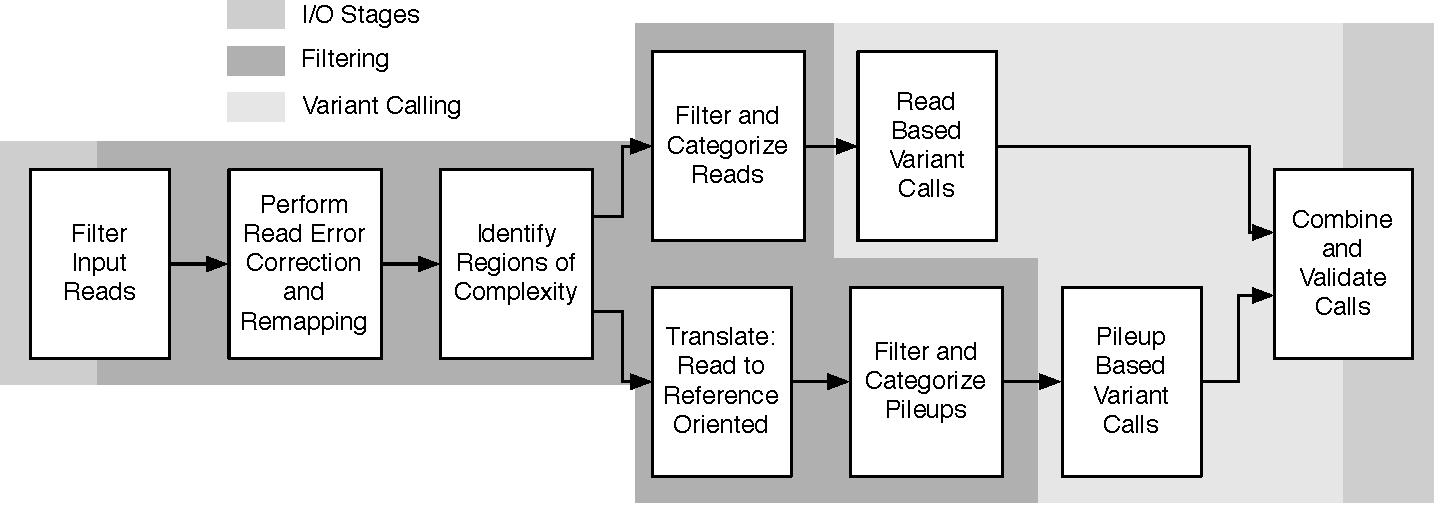
\includegraphics[width=0.9\linewidth]{avocado-architecture.pdf}
\end{center}
\caption{System architecture}
\label{fig:architecture}
\end{figure}

Logically, the system can be decomposed into three functions: input/out\-put, data filtering, and variant calling. The rest of this
section will give an overview of each of these three functions. The algorithms that support filtering and variant calling are not
discussed in this section --- instead, we will discuss them further in \S\ref{sec:filtering-calling}. We will also discuss how the
architecture of the system lends itself to easy extension.

\subsection{Input/Output}
\label{sec:io}

Although most variant calling tools take Sequence Alignment/Map (SAM\footnote{SAM is a plain-text based file format.In
practice, most tools use the Binary Alignment/Map (BAM) format. See Li et al.\cite{li09} for a discussion of the file formats.} files
as input and return Variant Call Format (VCF) files as output, we will use ADAM instead. ADAM provides several data structures for
genomics that are implemented under Avro and Parquet. Parquet is a columnar data store that stores data in compressed form.
When deserializing data, Parquet allows us to use predicates to only load relevant data. When these predicates are being used,
Parquet only decompresses the relevant field that must be checked --- if the predicate identifies the record, Parquet then
decompresses the full record. This predicate pushdown allows us to perform basic filtering when reading in the aligned
reads (e.g. only load reads whose quality is above a certain threshold), and should reduce the amount of I/O that we are performing.

We gain several additional advantages through the use of Avro. Avro allows us to define data structures using a markup
language. Once the data structure has been defined using the markup, it can be reused across most major programming
languages. By defining a straightforward data structure that is easily serialized and deserialized, we also eliminate the overhead
of needing to parse SAM/BAM files. We plan to update SNAP to support output using ADAM datatypes; in the meanwhile,
we can convert SAM/BAM files to ADAM through the use of the ADAM toolkit \cite{adam}.

A notable feature that we are implementing in ADAM for AVOCADO is pileup compression. Normally, reference oriented data is
stored in a conservative manner that retains full statistics for each base at the reference position. Instead, we plan to reduce the
data for like bases down into a single record. As a critical application for this variant caller is high-coverage (60$\times$) cancer
genomes, this may provide a significant reduction in the amount of data that needs to be distributed in our system, and may lead
to significant performance improvement.

\subsection{Data Filtering}
\label{sec:data-filtering}

One of the critical findings of the GQL project was that we can achieve a significant speedup in variant calling by eliminating
data that is unlikely to contain a structural variant \cite{kozanitis13}. In AVOCADO, we look to extend this approach further by treating
data filtering and segregation as a key part of successful variant calling. This work is predicated under several assumptions:

\begin{itemize}
\item With the exception of 10\% of the genome that contains high redundancy, structural variants can be called without
using based assembly techniques \cite{xia09}. For these remaining structural variants, there is a negligible accuracy
tradeoff that comes from using algorithms that increase statistical rigor at the cost of computation.
\item Within the remaining 90\% of the genome, the majority of loci do not contain evidence of structural variants and
can be discarded without significantly impacting accuracy \cite{kozanitis13}.
\item For the remaining regions that may contain evidence of variants, we can determine what sort of structural variant they
are likely to contain (SNP, short index), and optimize both accuracy and computational cost by picking algorithms tailored
to those specific structural variants.
\end{itemize}

We provision three stages for the filtering of data. As alluded to in \S\ref{sec:io}, we perform basic filtering on the input reads.
This first round of filtering will be based on the read quality. The second round of filtering will look to identify segments of the
genome which need to be called using read-assembly based methods. After this round of filtering, we segregate the genome
into two pipelines --- one for read-based identification, and another for pileup-based variant identification. In each of these
pipelines, we perform a third round of filtering that serves to pair reads/pileups with the algorithm that is most likely to successfully
identify their structural variant.

It is useful to note that data filtering may actually improve the accuracy of the variant calling system. In the preliminary work
done on the BIGGIE system, the authors found that filtering on complexity led to them making fewer incorrect SNP
calls~\cite{xia12}. This conclusion has logical backing: by looking for patterns in the base pair data, we can match
pileups/reads that exhibit evidence for a specific form of variant with algorithms that are optimized for correctly detecting
those variants.

\subsection{Variant Calling}
\label{sec:variant-calling}

As discussed in \S\ref{sec:data-filtering}, we plan to include several variant calling algorithms. At the moment, we plan to
implement the algorithms identified in Table \ref{tab:vc-algorithms}. A further discussion of these algorithms can be found
in \S\ref{sec:filtering-calling}.

\begin{table}[h]
\begin{center}
\caption{Variant Calling Algorithms}
\label{tab:vc-algorithms}
\begin{tabular}{| c | c |}
\hline
\bf Read Based & \bf Reference Based \\
\hline \hline
Local Assembly & SNP Calling \\
Long Indel & \\
Short Indel & \\
\hline
\end{tabular}
\end{center}
\end{table}

A consequence of having several different algorithms is that we will need to join the output of all algorithms at the end.
A na\"{i}ve approach is to pick the result generated by the ``most rigorous'' variant calling algorithm. However, since the
purpose of the filtering steps discussed in \S\ref{sec:data-filtering} is to send disparate segments of the genome to
different variant calling algorithms, there should not be any conflicting variant calls. More succinctly, if $VC_{k}$ is the
set of all variant calls made by algorithm $k$, we expect $VC_{i} \cap VC_{j} = \emptyset$ for all combinations of $i, j$.

\subsection{Extensibility and Scalability}
\label{sec:extensibility-and-scalability}

One of the inherent goals of this project is to produce a variant caller that has well defined interfaces and can easily be
extended. We hope that this will enable the rapid development and prototyping of future variant calling algorithms. From
a software engineering standpoint, we will achieve this by presenting clear interfaces for defining new filters and variant
calling algorithms for both read and pileup oriented data.

\subsection{Joint Variant Calling with Sufficient Statistics}
\label{sec:joint-variant-calling}

\section{Filtering and Calling Heuristics}
\label{sec:filtering-calling}

\subsection{Local Assembly}
\label{sec:local-assembly}

Local assembly will be used in areas of high genomic complexity\footnote{These can be areas with long sequence
repeats, areas that are redundant/repeated in the genome, or areas with large structural variants.} to perform very accurate
structural variant calling. It is useful to note that this the highest accuracy method used in the GATK's HaplotypeCaller.

There are several heuristics that can be used for identifying high genomic complexity. A primary heuristic is read mapping
quality --- if there are many reads that are poorly mapped, this can indicate that the location has high similarity to other
regions in the genome and is hard to differentiate, or that the reads are mapping poorly to the reference due to a structural
anomaly in the sequenced genome. As a base heuristic, we will look for sliding windows of $n$-bases with low Phred scores.
These parameters can be adjusted by the user --- as defaults, we can set $n = 150$ and Phred $= 30$.

\subsection{Long Indel}
\label{sec:long-indel}

For long deletion detection, we may be able to implement an algorithm similar to the split-read\footnote{Reads where
there is no contiguous alignment/mapping.} based algorithm implemented by BreakDancer~\cite{chen09}. This
algorithm provides highly accurate detection of long deletions, at a lower computational cost than local assembly.
However, currently SNAP does not perform split-read alignment~\cite{zaharia11}. Later in the project, we may
look to extend SNAP, or to evaluate the algorithm with aligned reads from an aligner that performs split-read based
alignment.

\subsection{Short Indel}
\label{sec:short-indel}

Here, we define a short indel as an insertion or deletion less than 100 base pairs long. As indicated in Chen et al.
\cite{chen09}, the Smith-Waterman sequence alignment algorithm (see~\cite{smith81}) can be used for accurately
identifying short indels. To call these variants, we perform a consensus Smith-Waterman:

\begin{enumerate}
\item Using primary read alignments, find areas with evidence of short indels.
\item Find all reads with a primary alignment that overlaps this area, along with an additional padding of $w$. The total
overlapping region will be from $b - w$ to $e + w$, where $b, e$ are the beginning and end of the area where there is
evidence for an indel.
\item Per read, create a scoring matrix against the reference ($S_i$).
\item Reduce all scoring matrices by performing an elemental sum, weighted by the error probability of the read
($\epsilon_i$):
$$
S [x, y] = \sum_i (1 - \epsilon_i) * S_i [x,y] , \forall x, y
$$
\item Perform conventional Smith-Waterman backtracking on this final scoring matrix.
\end{enumerate}

As has been noted, the Ukkonen algorithm for string matching is more efficient than the Smith-Waterman
algorithm~\cite{ukkonen85}. This is the algorithm used in SNAP~\cite{zaharia11}. I am currently looking into the SNAP
code to identify whether any algorithmic changes would need to be made to use Ukkonen's algorithm in place of
Smith-Waterman.

\subsection{SNP Calling}
\label{sec:SNP-calling}

To perform SNP calling, we first identify the likely genotype class\footnote{For diploid human, classes include homozygous
matching reference, heterozygous with one base matching reference, or no bases matching reference.} using equation~(2)
from Li et al \cite{li11}. We will filter pileups on the basis of whether they contain any mismatches --- only pileups that contain
a mismatch will be evaluated.

\section{Experimental Validation}
\label{sec:experimental-validation}

We plan to validate this tool using the SMASH benchmarking suite \cite{talwalkar13}. This benchmarking suite will allow us to
compare both performance and accuracy against other high quality variant calling engines.

\subsection{Parallel vs. Distributed}
\label{sec:parallel-vs-distributed}

This system can be implemented either as a traditional parallel program on a single machine, or as a distributed application
running on a cluster. It is useful to note that SNAP \cite{zaharia11} chose to run on a single machine. Our general implementation
is task parallel between the read/reference-oriented calling, and also between algorithms within these two sections. For the
variant calling algorithms themselves, the Short Indel and SNP callers are clearly data parallel.

Since our algorithms have a high level of parallelism, our scaling on parallel and distributed system should be determined solely
by the amount of data that needs to be moved between processors/machine. We hope that the filtering steps we employ will
minimize data transfer and improve scalability.

We will likely encounter a tradeoff between efficiency and performance when scaling from a parallel system running on a single
machine to a distributed system running on a cluster. This opens us up to several tradeoffs that we can investigate --- specific
tradeoffs of interest might include finding the minimal cost configuration for variant calling, or finding the system that provides
the lowest end-to-end latency (independent of cost or scaling efficiency).

\subsection{Computational Cost of Joint Variant Calling}
\label{sec:computational-cost-joint}

One of the major contributions of our work is that we plan to calculate population statistics offline and catalog them in a database.
The GATK \cite {mckenna10} and SAMtools \cite{li11} both implement population statistics calculation as an online operation. The
impact of performing joint variant calling in this manner is that if a single sample is added to a population, the entire population
must be reanalyzed before calling variants on this single sample. This has significant cost for large populations, and we hope to
replace this large cost that grows with population size with a single, fixed latency cost. With this feature, we will need to characterize
the tradeoff at which it becomes more performant to perform offline calculation, as well as any accuracy impact of performing offline
analysis.

\subsection{Order of Work}
\label{sec:order-of-work}

We plan to conduct our work in the following order:

\begin{itemize}
\item In parallel, we will implement:
\begin{enumerate}
\item SNP Calling (see \S\ref{sec:SNP-calling})
\item Local assembly (see \S\ref{sec:local-assembly})
\item Sufficient statistics calculation (see \S\ref{sec:joint-variant-calling})
\end{enumerate}
\item Joint variant calling for SNPs using sufficient statistics (see \S\ref{sec:joint-variant-calling})
\item Short Indel detection (see \S\ref{sec:short-indel})
\item Long Indel detection (see \S\ref{sec:long-indel}) using a split-read aligner
\item Enhancements to SNAP to add the ability to perform split-read alignment
\item Joint variant calling for structural variants (see \S\ref{sec:joint-variant-calling})
\end{itemize}

\small

\bibliographystyle{acm}

\bibliography{avocado-proposal}

\end{document}
